% !TeX root = ../main.tex

\chapter{整体设计}
\label{cha:chapter02}
本项目选择把跳跃和滑翔分开作为两个独立的过程来分析与控制,用一个无刷电机驱动跳跃部分,用一个舵机控制机翼的开合。
\section{理论计算}
\label{sec:calculations}
取$g=9.8m/s^2$,预计机器人重量$m=200g$,跳跃高度$h=1m$,起跳电机做功时间$t=0.1s$,则机器人所需最小动能:
\begin{equation}
\label{equ:chap2:W_calc}
W_k=mgh
\end{equation}
二级齿轮减速器机械效率估计为$\eta=80\%$,则所需电机输出最小平均功率:
\begin{equation}
  \label{equ:chap2:P_calc}
  \bar{P}_{min}=\frac{W_k}{t·\eta}
  \end{equation}
解得:$$\bar{P}_{min}=24.5(W)$$
二级齿轮减速器减速比大约在10\sim30:1,设计中一次起跳输出级齿轮大约需要转半圈,取减速比20:1,则所需无刷电机转速:
$$\omega_{min}=0.5\times10\div t\times60=6000(rpm)$$
使用2S锂离子电池,额定电压$V=7.4V$,则所需最小电机KV值:
$$KV_{min}=\omega_{min}\div V=810(rpm/V)$$
一般来讲KV值越小无刷电机转矩越大,根据计算及机械需求考虑,选择了最大功率$P_{max}=168W$的朗宇X2305航模无刷电机,KV值$KV=1450$。\\
机器人起跳最小速度:
\begin{equation}
  \label{equ:chap2:v_calc}
  v=\sqrt{2gh}
  \end{equation}
根据动量定理:
\begin{equation}
  \label{equ:chap2:motion_principle}
  \bar{F}·t=m·v
  \end{equation}
解得所需平均力:$$\bar{F}=8.854(N)$$
航模用无刷电机的力矩数据不好获得,我们通过相同工作条件下的带螺旋桨升力进行估算,实际输出力只会更大。电机参数显示6000rpm时的升力等效质量约为$m_f=200\sim300g$,即经减速器输出的力为:$$F_min=m_{f,min}·g·20=39.2(N)>\bar{F}$$
此处还未考虑腿部连杆结构带来的机械增益,而其均值应>1,因此理论上输出力是足够支持跳跃的。
\section{元件选型}
\label{sec:components}
根据上述计算过程与现实考量,选择元件如表\ref{tab:bom}所示。
\begin{table}[htb]
  \centering
  \begin{minipage}[t]{0.8\linewidth}
  \caption{BOM表}
  \label{tab:bom}
    \begin{tabularx}{\linewidth}{lX}
      \toprule[1.5pt]
      {\heiti 元件名} & {\heiti 描述} \\\midrule[1pt]
      朗宇X2305无刷电机 & 外转子无刷电机,KV值1450 \\
      NanoPi Duo2 开发板 & 全志H3主控,运行Ubuntu 18.04\\
      FOC电机控制板 &  基于STSPINF0A方案的BLDC矢量控制 \\
      EMAX 2S航模锂电池 & 容量300mAh,质量为15g\\
      DS-S002M 4.3g数字舵机 & 用于控制机翼开合\\
      OV5640摄像头 & 500W像素,1080p@30fps,720p@60fps\\
      \bottomrule[1.5pt]
    \end{tabularx}
  \end{minipage}
\end{table}
\section{机械设计}
\label{sec:mechanical}
初步设计的机器人整体结构三维仿真图如下(螺丝等固定细节略去):
\begin{figure}[H]
  \centering
  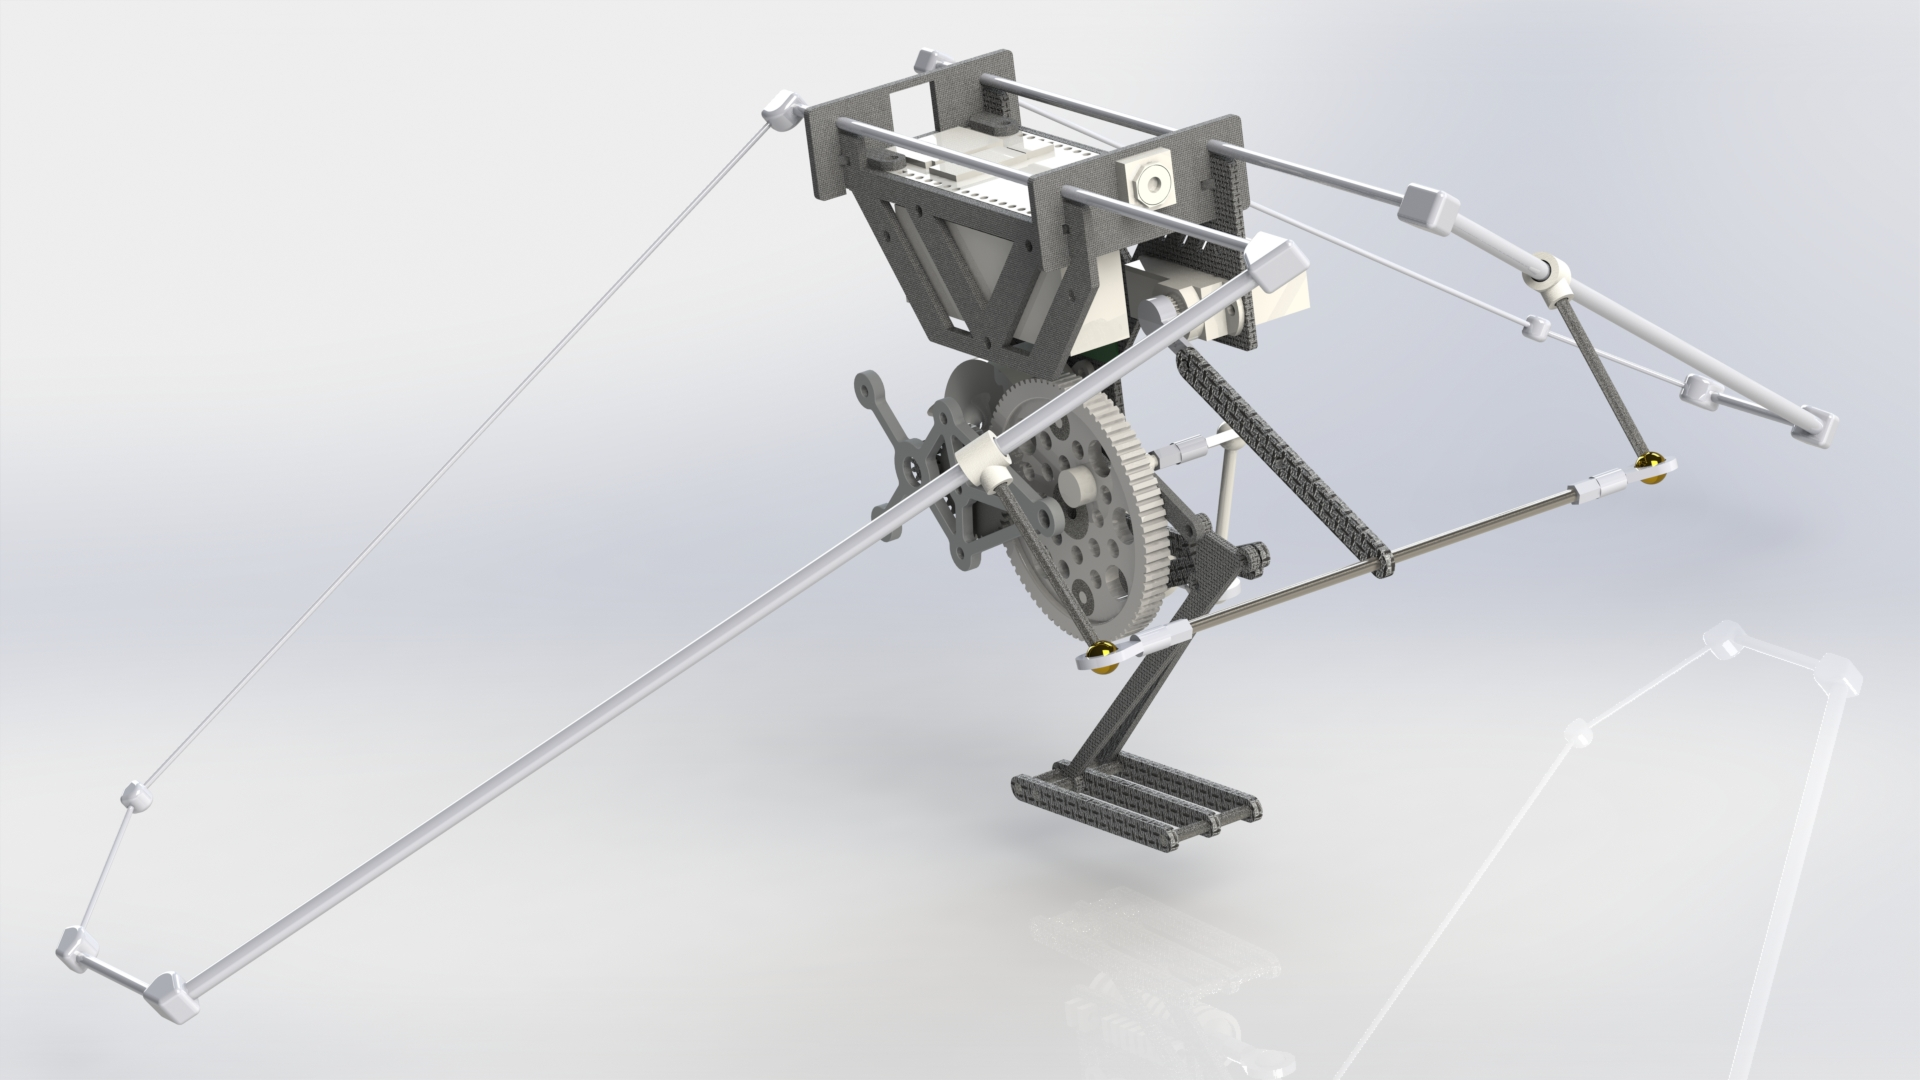
\includegraphics[height=8cm]{render2.jpg}
  \caption{整体结构渲染图}
  \label{fig:render_v1}
\end{figure}
\subsection{减速器设计}
设计目标为减速比20:1的两级齿轮减速器。考虑本项目实际尺寸,选用模数为0.5或0.6的齿轮较为合适。在市面上可直接买到的齿轮中,选择了0.5模数15齿的主轴齿轮,10/36齿的次级双层齿轮和80齿的末级齿轮。

\subsection{腿部设计}
参考Salto\cite{Salto}的腿部模型,此处实现了如图\ref{fig:2d_leg}所示的连杆结构。其中灰色圆为输出级齿轮,带动上部的曲柄-摇臂四连杆结构,同时四连杆摇臂为一凹四边形块,与机身相连的另一点在下部又组成了一个平行四边形四连杆,在输出级利用杠杆结构增大位移,实现触地端的较大速度,从而使身体跳起。虽然看上去略显复杂,但总体形态接近自然界大多数生物的腿部构造,这也从一个侧面反映了该结构的合理性。

\begin{figure}[H]
  \centering%
  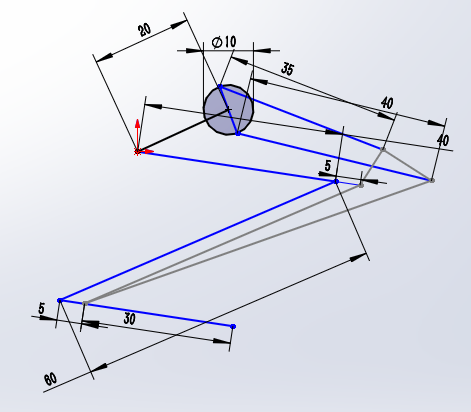
\includegraphics[height=6cm]{2d_leg_fold.png}
  \caption{起跳前准备姿势}
  \label{fig:2d_leg_fold}
\end{figure}
\begin{figure}[H]
  \centering%
  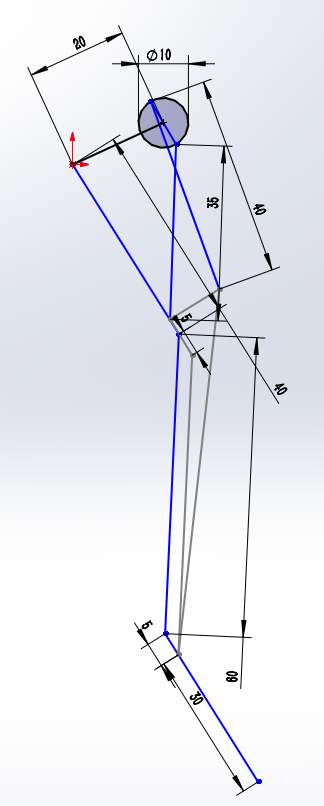
\includegraphics[height=11cm]{2d_leg_stretch.png}
  \caption{起跳后空中姿势}
  \label{fig:2d_leg_stretch}
\end{figure}

据此尺寸在SolidWorks中设计出三维模型,装配示意图如图\ref{fig:3d_leg}所示。
\begin{figure}[H]
  \centering%
  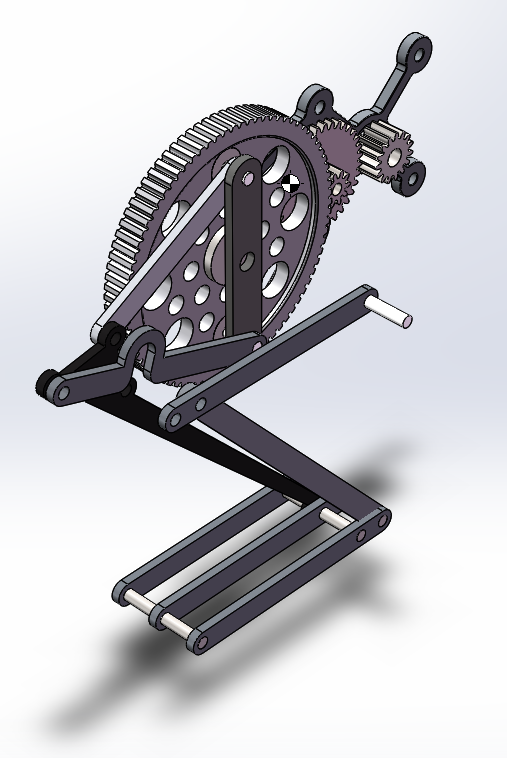
\includegraphics[height=8cm]{3d_leg.png}
  \caption{腿部装配图}
  \label{fig:3d_leg}
\end{figure}

\subsection{插图}
\label{sec:graphs}

强烈推荐《\LaTeXe{} 插图指南》!关于子图形的使用细节请参看 \pkg{subcaption} 宏包的说明文档。

\subsubsection{一个图形}
\label{sec:onefig}
一般图形都是处在浮动环境中。之所以称为浮动是指最终排版效果图形的位置不一定与源文
件中的位置对应\footnote{This is not a bug, but a feature of \LaTeX!},这也是刚使
用 \LaTeX{} 同学可能遇到的问题。如果要强制固定浮动图形的位置,请使用 \pkg{float} 宏包,
它提供了 \texttt{[H]} 参数,比如图~\ref{fig:xfig1}。
\begin{figure}[H] % use float package if you want it here
  \centering
  
\includegraphics{thu-whole-logo.pdf}
  \caption{利用 Xfig 制图}
  \label{fig:xfig1}
\end{figure}

大学之道,在明明德,在亲民,在止于至善。知止而后有定;定而后能静;静而后能安;安
而后能虑;虑而后能得。物有本末,事有终始。知所先后,则近道矣。古之欲明明德于天
下者,先治其国;欲治其国者,先齐其家;欲齐其家者,先修其身;欲修其身者,先正其心;
欲正其心者,先诚其意;欲诚其意者,先致其知;致知在格物。物格而后知至;知至而后
意诚;意诚而后心正;心正而后身 修;身修而后家齐;家齐而后国治;国治而后天下
平。自天子以至于庶人,壹是皆以修身为本。其本乱而未治者否矣。其所厚者薄,而其所
薄者厚,未之有也!

\hfill —— 《大学》


\subsubsection{多个图形}
\label{sec:multifig}

如果多个图形相互独立,并不共用一个图形计数器,那么
用 \texttt{minipage} 或者\texttt{parbox} 就可以。否则,请参看
图~\ref{fig:big1-subcaptionbox},它包含两个小图,分别是图~\ref{fig:subfig1}和
图~\ref{fig:subfig2}。推荐使用 \cs{subcaptionbox},因为可以像
图~\ref{fig:big1-subcaptionbox} 那样对齐子图的标题,也可以使用 \pkg{subcaption}
宏包的 \cs{subcaption}(放在 minipage中,用法同\cs{caption})或
是 \pkg{subfigure} 、\pkg{subtable}环境,像图~\ref{fig:big1-subfigure},不要再
用 \cs{subfloat}、\cs{subfigure} 和 \cs{subtable}。

\begin{figure}[h]
  \centering%
  \subcaptionbox{第一个小图形\label{fig:subfig1}}[3cm] %标题的长度,超过则会换行,如下一个小图。
    {
\includegraphics[height=3cm]{thu-fig-logo.pdf}}%
  \hspace{4em}%
  \subcaptionbox{第二个小图形,注意这个图略矮些。如果标题很长的话,它会自动换行\label{fig:subfig2}}
      {
\includegraphics[height=2cm]{thu-text-logo.pdf}}
  \caption{包含子图形的大图形(subcaptionbox示例)}
  \label{fig:big1-subcaptionbox}
\end{figure}
\begin{figure}[h]
  \centering%
  \begin{subfigure}{3cm}
    
\includegraphics[height=3cm]{thu-fig-logo.pdf}
    \caption{第一个小图形}
  \end{subfigure}%
  \hspace{4em}%
  \begin{subfigure}{0.5\textwidth}
    
\includegraphics[height=2cm]{thu-text-logo.pdf}
    \caption{第二个小图形,注意这个图略矮些。subfigure中同一行的子图在顶端对齐。}
  \end{subfigure}
  \caption{包含子图形的大图形(subfigure示例)}
  \label{fig:big1-subfigure}
\end{figure}

古之学者必有师。师者,所以传道受业解惑也。人非生而知之者,孰能无惑?惑而不从师,
其为惑也,终不解矣。生乎吾前,其闻道也固先乎吾,吾从而师之;生乎吾後,其闻道也亦
先乎吾,吾从而师之。吾师道也,夫庸知其年之先後生於吾乎!是故无贵无贱无长无少,道
之所存,师之所存也。

嗟乎!师道之不传也久矣,欲人之无惑也难矣。古之圣人,其出人也远矣,犹且从师而问焉;
今之众人,其下圣人也亦远矣,而耻学於师。是故圣益圣,愚益愚。圣人之所以为圣,愚
人之所以为愚,其皆出於此乎?爱其子,择师而教之,於其身也,则耻师焉,惑焉。彼童子
之师,授之书而习其句读者,非吾所谓传其道、解其惑者也。句读之不知,惑之不解,或师
焉,或不焉,小学而大遗,吾未见其明也。巫医、乐师、百工之人不耻相师,  士大夫之族
曰“师”曰“弟子”之云者,则群聚而笑之。问之,则曰:彼与彼年相若也,道相似也,位
卑则足羞,官盛则近谀。呜呼!师道之不复,可知矣。巫医、乐师、百工之人。吾子不齿,
今其智乃反不能及,其可怪也欤!圣人无常师。孔子师郯子、苌子、师襄、老聃。郯子之徒,
其贤不及孔子。孔子曰:“三人行,必有我师。”是故弟子不必不如师,师不必贤於弟子。
闻道有先後,术业有专攻,如是而已。

如果要把编号的两个图形并排,那么小页就非常有用了:
\begin{figure}
\begin{minipage}{0.48\textwidth}
  \centering
  
\includegraphics[height=2cm]{thu-whole-logo.pdf}
  \caption{并排第一个图}
  \label{fig:parallel1}
\end{minipage}\hfill
\begin{minipage}{0.48\textwidth}
  \centering
  
\includegraphics[height=2cm]{thu-whole-logo.pdf}
  \caption{并排第二个图}
  \label{fig:parallel2}
\end{minipage}
\end{figure}

李氏子蟠,年十七,好古文、六艺,经传皆通习之,不拘於时,学於余。余嘉其能行古
道,作师说以贻之。

\hfill —— 韩愈(唐)
